\begin{column}{\onecolwid} % The first column



\begin{block}{Summary}

Datasets such as the TARGET collection of pediatric cancer samples and the Kaviar database of known variants contain variant calls from Illumina and Complete Genomics platforms. Platform differences make integrating variants for cross platform analysis difficult. Here we use Kaviar to investigate platform differences when calling small insertions and deletions (indels). We search for annotated genomic features (repetitive elements, blacklist regions, etc) that predict platform differences, and use the convolutional neural network architecture provided by pysster \cite{budach2018pysster} to integrate sequence motifs and annotated genomic features to build a classifier of Complete Genomics indels that predicts their verification status in Illumina data. We find that sequence motif features generalize to a validation indel set better than a combination of annotated genomic features.

\end{block}

\begin{block}{Kaviar data}

%------------------------------------------------

\begin{figure}
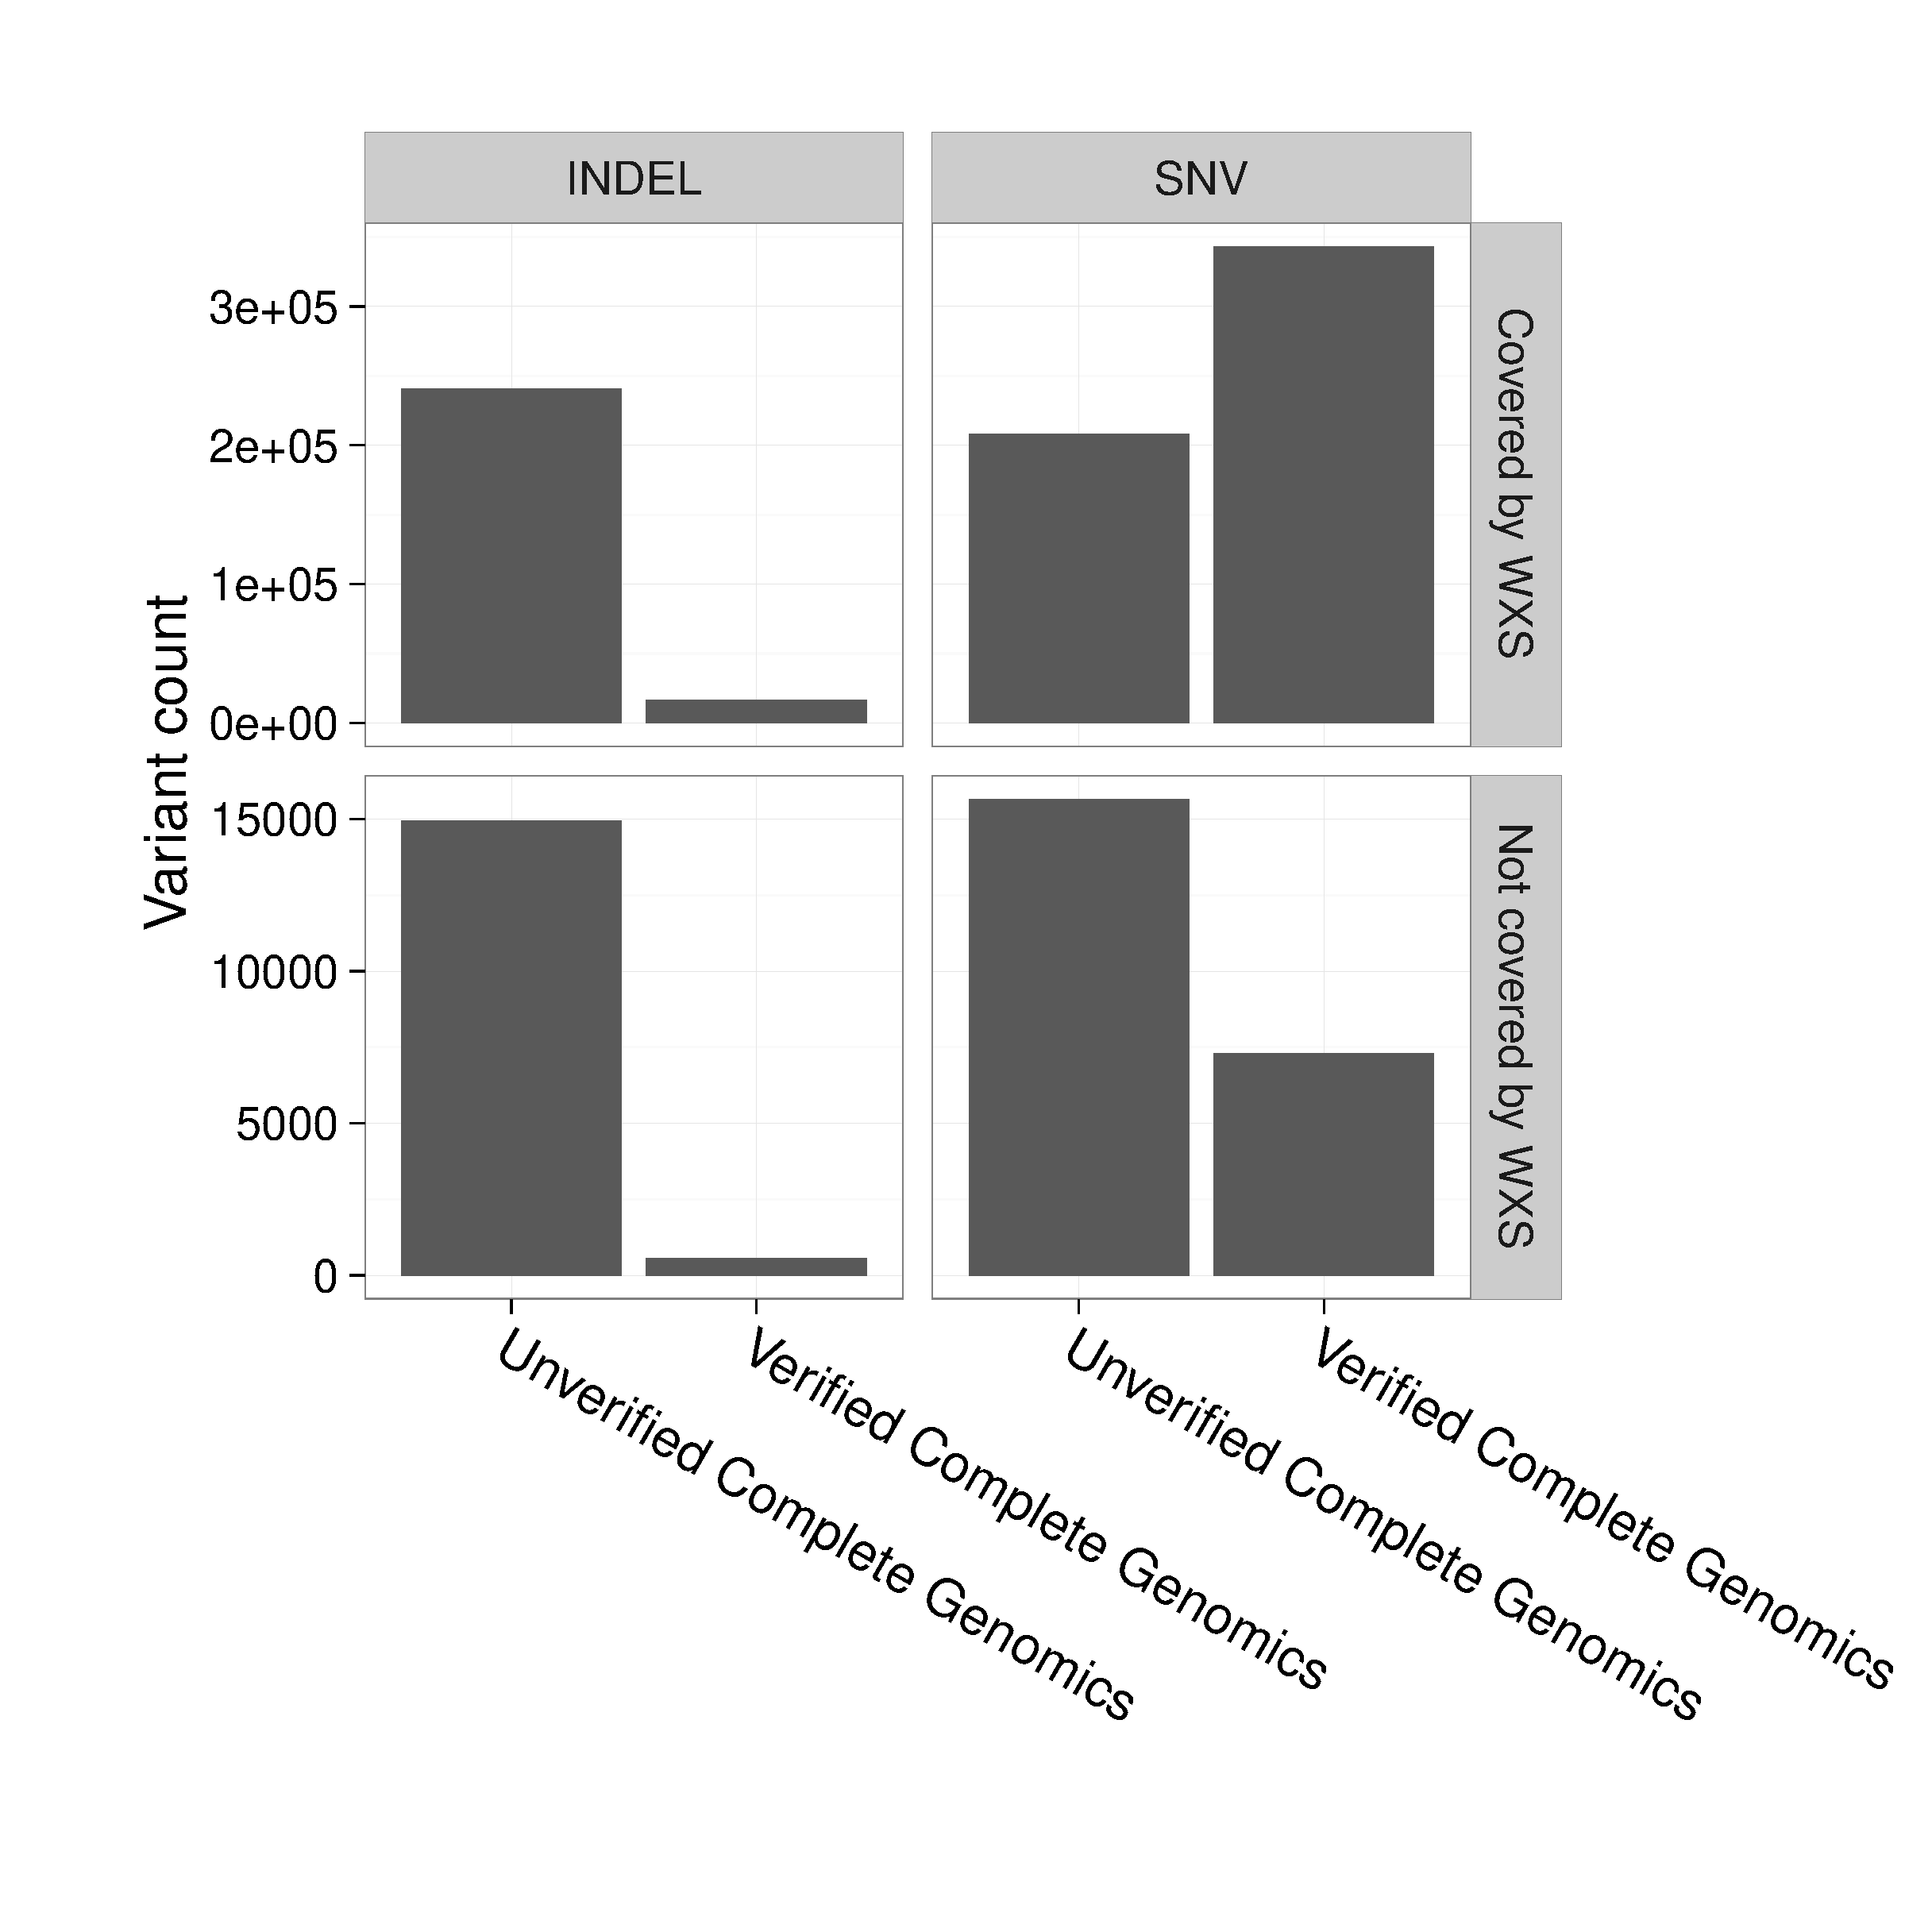
\includegraphics[width=1\linewidth]{figs/init_counts.eps}
\end{figure}

\begin{alertblock}{Kaviar indels}
Pysster training and validation indels: 8105 verified Complete Genomics indels, and 8230 unverified Complete Genomics indels. External validation indels: 55 validated Complete Genomics indels, and 102,535 unvalidated Complete Genomics indels.
\end{alertblock}

\end{block}


%----------------------------------------------------------------------------------------

\end{column} % End of the first column